\chapter{Preface/Acknowledgements}
The preface contains a short description of the topic; words of thanks to companies, mentors, supervisors, family members, etc., for their support are optional under consideration of relevant data protection terms.

\section{Using this template}
This document is a template and contains optional lists. Lists that are not required (list of abbreviations, glossary, list of figures, list of tables and list of equations) may be deleted after consultation with your supervisor. Please discuss with your supervisor in advance which format, reference style, structure of chapters, etc. is to be used. Course-specific regulations might be included in an additional document. Please contact your supervisor on this matter.
\vspace{6pt}\\
The examples provided in this template are for your information only. Replace them with your own text after reading them carefully. Delete unnecessary information. Please keep in mind that automatic numbering is shown correctly in the document as a whole only after you have deleted sub-chapters of the preface which explains the template.
\vspace{6pt}\\
For an updated table of contents, the document should always be compiled twice.
\vspace{6pt}\\
\textcolor{red}{\textbf{The present format template was prepared to the best of our knowledge and judgement. However, it is used at the users’ own risk with regard to the possible loss of data, computer problems or financial and material damage which may result from the use of this template. The authors of the present format template and the University of Applied Sciences Upper Austria do not accept any liability for the correct functionality of this template.}}



\newpage
\subsection{Experience with \LaTeX}
Some experience with the software package {\LaTeX} is necessary for using this template. The program \textbf{TeXstudio} (\url{www.texstudio.org}) and the windows distribution \textbf{MiKTEX} (\url{www.miktex.org}) were used to create this template. Problems may arise when using other software. This template is not compatible with Apple operating systems.\\
The style packages used and the commands needed are not explained in this template. Detailed help for the commands is offered at the internet in many forums and websites.

\section{Headings}
With respect to headings, consider the following points for the formulation of a table of contents:
\begin{itemize}
	\item Do not use unknown abbreviations in headings
	\item No full stop at the end of headings
	\item Make sure that a heading – without associated text – is not situated on the last line of a page; a page should also not start with a single line which belongs to the paragraph on the previous page.
	\item The degree of detail corresponds to the focus and emphasis of the thesis
	\item Always use at least two sub-chapters in one chapter; otherwise do not use sub-chapters
	\item Use a maximum of 5 levels of sub-chapters
\end{itemize}
Due to the automatic structuring done by {\LaTeX} the headings can not be illustrated here, but the commands can be explained:
\begin{itemize}
	\item level of heading 1: \verb|\chapter{...}| command
	\item level of heading 2: \verb|\section{...}| command
	\item level of heading 3: \verb|\subsection{...}| command
	\item level of heading 4: \verb|\subsubsectin{...}| command
	\item level of heading 5: \verb|\paragraph{...}| command
\end{itemize}

\newpage
\section{Abbreviations}
{\LaTeX} automatically creates spaces between characters in some cases. For common abbreviations to be depicted in the right way, commands are defined.

\begin{multicols}{2}	
	\begin{itemize}
		\item Command: \verb|\mn|\dotfill\mn
		\item Command: \verb|\mx|\dotfill\mx
		\item Command: \verb|\etc|\dotfill\etc
		\item Command: \verb|\ie|\dotfill\ie
		\item Command: \verb|\eg|\dotfill\eg
		\item Command: \verb|\cf|\dotfill\cf
	\end{itemize}
\end{multicols}

\newpage
\section{Figures}
\label{sec: Figures}
The figure environment has to be used for inserting and referencing figures.\\
A figure can be inserted with the following lines of code:
\begin{figure}[h]
	\centering
	
\includegraphics[width=0.50\textwidth]{FH.png}
	\caption{Example of inserting a figure}
	\label{fig: ExampleFigure-1}
\end{figure}\\
Two figures next to each other with one caption can be inserted with the following commands:
\begin{figure}[htp!]
	\begin{minipage}[t]{0.49\textwidth}
		\centering
		
\includegraphics[width=0.49\textwidth]{FH.png}
	\end{minipage}
	\hfill
	\begin{minipage}[t]{0.49\textwidth}
		\centering
		
\includegraphics[width=0.49\textwidth]{FH.png}
	\end{minipage}
	\caption{Example of two figures with one caption}
	\label{fig: ExampleFigure-2}
\end{figure}\\
Two figures next to each other with separate captions can be inserted with the commands below:
\begin{figure}[htp!]
	\begin{minipage}[t]{0.49\textwidth}
		\centering
		
\includegraphics[width=0.49\textwidth]{FH.png}
		\caption{Examples of two figures with separate captions}
		\label{fig: ExampleFigure-3}
	\end{minipage}
	\hfill
	\begin{minipage}[t]{0.49\textwidth}
		\centering
		
\includegraphics[width=0.49\textwidth]{FH.png}
		\caption{Examples of two figures with separate captions}
		\label{fig: ExampleFigure-4}
	\end{minipage}
\end{figure}\\
Consider the following points when using figures:
\begin{itemize}
	\item Figures must be referenced within or linked to the text; otherwise they are superfluous. To do this, use the command \verb|\ref{}|
	[see Fig.~\ref{fig: ExampleFigure-1}]\\
	An additional page reference can be added with the command \verb|\pageref{}| \newline
	[see Fig.~\ref{fig: ExampleFigure-1} on page \pageref{fig: ExampleFigure-1}]
	\item Not every figure needs to be in the text. Analyses, tables, backup information, \etc can be collected in the appendix. However, the text should reference them.
	\item If necessary, add a legend in the figures and the necessary references.
\end{itemize}

\newpage
\section{Tables}
Tables must be referenced within or linked to the text [see Table \ref{tab: ExampleTable-1} on page~\pageref{tab: ExampleTable-1}].\\
Using the table environment, tables can be numbered and referenced correctly.\\
A table can be inserted in two different ways.
\subsection{Insert as a figure}
An image of a table can be inserted in the table environment.
\begin{table}[h]
	\centering
	\caption{Example of a table inserted as a figure}
	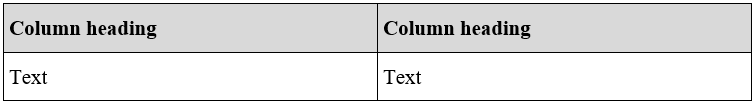
\includegraphics[scale=0.6]{0000_Testtabelle.png}
	\label{tab: ExampleTable-1} 
\end{table}
\subsection{Insert as a table}
It is possible to create tables with {\LaTeX} directly.
\begin{table}[h]
	\centering
	\caption{Example of a table which is created in \LaTeX}
	\begin{tabular}{c|c||c|}
		Column heading & Column heading & Column heading \\
		\midrule[2pt]
		1 & Test-1 & Test-2\\ 
		\hline 2 & 0 & 0  \\ 
		3 & 0 & 0  \\ 
		4 & 0 & 1  \\
		\hline 
	\end{tabular}
	\label{tab: ExampleTable-2} 
\end{table}

\section{Equations}
Usually, equations are integrated into sentences (example $e=m\cdot c^2$). They may form part of the main body of the text or be written separately on their own line or in their own paragraph. In the latter case, an equation like
\begin{align}
	e=m\cdot c^2
	\label{eq: ExampleEquation-1}
\end{align}
may be numbered and the relevant number can be used to refer back to the equation later in the text. Example of a cross-reference: see Equation \ref{eq: ExampleEquation-1} on page \pageref{eq: ExampleEquation-1}).
\vspace{6pt}\\
Further examples for embedding equations:
\\
Newton's law $F=ma$ is one of the most important laws of nature.
\\
The general form of a Fourier series reads
%
\begin{align}
f(x)=a_0 +\sum_{n=1}^\infty \left( a_n \cos\frac{n\pi x}{L} + b_n \sin\frac{n\pi x}{L} \right) .
\label{eq: Formel2}
\end{align}
%
Herein, $a_n$ and $b_n$ are denoted as Fourier coefficients. Notice the punctuation mark
in Equation~\ref{eq: Formel2}!

\begin{comment}

\section{Referencing other sources}
For citations, you are free to choose one of the following options:
\begin{itemize}
	\item insert citations manually;
	\item insert citations using a bibliographic software.
\end{itemize}
The main point for you is to enter all citations and literature references correctly, \ie according to section \ref{sec: TypeOfCitation} on page \pageref{sec: TypeOfCitation} and section \ref{sec: Bibliography} on page \pageref{sec: Bibliography}, respectively. Agree with your supervisor how to reference sources and to use citation templates when you start working on your thesis. Using citation templates may necessitate manual modifications before you submit your thesis.\\
A *.bib file is necessary to generate a bibliography in {\LaTeX}. There are several options to create such a file (manually, using the program JabRef, \dots).

\subsection{Important notes on referencing}
\begin{itemize}
	\item Direct quotations (usually with quotation marks) and indirect quotations (without quotation marks) are distinguished.
	\begin{addmargin}[10pt]{0pt}
		{\footnotesize Every citation must be verifiable and correctly documented. The correct use of citations is an expression of scientific accuracy. Ideas taken from outside sources are always to be marked clearly as a citation – regardless of whether direct or indirect quotation.\footnote{Translated from Karmasin/Ribing, 2019, p. 114.}}
	\end{addmargin} 
	\item Integrate short direct quotations within the main body of the text. For direct quotations exceeding three lines in regular formatting, use the following template. Quotation marks are not used in this case:
	\begin{addmargin}[10pt]{0pt}
		{\footnotesize Lorem ipsum dolor sit amet, consectetuer adipiscing elit. Maecenas porttitor congue massa. Fusce posuere, magna sed pulvinar ultricies, purus lectus malesuada libero, sit amet commodo magna eros quis urna. Nunc viverra imperdiet enim. Fusce est. Vivamus a tellus. Pellentesque habitant morbi tristique senectus [\dots] fames ac turpis egestas. Proin pharetra nonummy pede. \cite[p.~6]{Meier:Globalisierung}}
	\end{addmargin} 
	\item ``Plagiarism is not only a direct quotation without quotation marks, but also an indirect quotation presented as if it was derived from one’s own findings.''\footnote{Translated from ibid.}
	\item Quotations immediately following a heading should only be used in exceptional cases.
	\item The content of citations must not be changed.
	\item All statements without (a) reference(s) are your own point of view, findings or generally known facts.
	\item Translations must be indicated in a footnote.
	\item Numbers have scientific relevance only if they can be verified. Thus, a reference is always needed when numbers are presented.
\end{itemize}
\subsection{Using direct and indirect quotations}
\begin{itemize}
	\item Texts taken word for word from the source must always be in quotation marks, except for block quotations [see above]. Always use the English quotation marks \mbox{(`` '')}, not the German quotation marks (\glqq{} \grqq) to highlight a quotation. If a quotation already contains quotation marks, change it into single quotation marks (` '):
	\begin{addmargin}[10pt]{0pt}
		\textcolor{red}{Müller writes: ``In the old days, the authorities had the financial power `firmly' in their grasp'' [Müller, 2010, p. 5].}
	\end{addmargin}
	\item Your own additions and amendments must be put in square brackets. The content of the citation must not be changed:
	\begin{addmargin}[10pt]{0pt}
		\textcolor{red}{According to Müller, ``in the old days, the authorities [had] the financial power [\dots]'' [Müller, 2010, p. 5].}
	\end{addmargin}
	\item Omission of one or several words is indicated by three dots in square brackets. Ellipses can be inserted with the command \verb|\dots| (do not use three full stops!):
	\begin{addmargin}[10pt]{0pt}
		\textcolor{red}{``In the old days, the authorities [\dots]'' [Müller, 2010, p. 5].}
	\end{addmargin}
	\item For indirect quotations, indication of the source without citation marks is sufficient:
	\begin{addmargin}[10pt]{0pt}
		\textcolor{red}{According to Müller, the authorities had control over the finances [\cf Müller, 2010, p. 5].}
	\end{addmargin}
	\item Repetition of the same citation can be marked with \textit{ibid}. However, there must be a direct connection to the reference:
	\begin{addmargin}[10pt]{0pt}
		\textcolor{red}{According to Müller, the authorities had control over the finances [\cf Müller, 2010, p. 5]. The lower classes did not have any power [\cf ibid., p. 7].}
	\end{addmargin}
\end{itemize}

\subsection{Different types of citations}
\label{sec: TypeOfCitation}
Talk to your supervisor to agree upon the types of citation to be used.

\subsubsection{Reference within the text (AGR, AT, MB, PDK)}
Meier claims that this aspect is important~\citeauthoryear[\cf][p.~5]{Meier:Globalisierung}.\newline
Meier says that ``this point [\dots] is relevant''~\citeauthoryear[p.~5]{Meier:Globalisierung}.\newline
This is also in line with more recent literature~\citeauthoryear[\cf][p.~10]{Mueller:Meier}.\newline
An overview of current research was published recently~\citeauthoryear[\cf][pp.~20-35]{Mueller:Meier:Huber}.\newline
Earlier academic publications had mentioned this topic as a research gap~\citeauthoryear[\cf][p.~85]{Mueller:Meier:Huber:Tausch}.\newline
“Placeholder text for a direct quotation from an AI tool” \citeauthoryear{OpenAI:2023}.\newline
Placeholder text for an indirect quotation from an AI tool \citeauthoryear[\cf][]{OpenAI:2023}.\newline
\underline{BibStyle}: \textsf{FHWelsAlphabeticBrackets}

\subsubsection{Reference within the text (BI, BUT, IPM, LCW, LTE)}
Meier claims that this aspect is important (Meier, 2011, p. 5).\newline
Meier says that “this point […] is relevant” (Meier, 2011, p. 5).\newline
This is also in line with more recent literature (Müller and Meier, 2019, p. 10).\newline
An overview of current research was published recently (Müller, Meier and Huber, 2021, pp. 20-35).\newline
Earlier academic publications had mentioned this topic as a research gap (Müller et al., 2016, p. 85).\newline
“Placeholder text for a direct quotation from an AI tool” (OpenAI, 2023). \newline
Placeholder text for an indirect quotation from an AI tool (OpenAI, 2023).\newline
\underline{BibStyle}: This citation style is not represented in the Latex template. To cite with the
\verb|\cite| command, the style files have to be adapted accordingly!

\subsubsection{Reference in the footnote (AMM, MEWI)}
Meier claims that this aspect is important.\footciteauthoryear[\Cf][p.~5]{Meier:Globalisierung}\newline
Meier says that ``this [\dots] point is relevant''.\footciteauthoryear[p.~5]{Meier:Globalisierung}\newline
This is also in line with more recent literature.\footciteauthoryear[\Cf][p.~10]{Mueller:Meier}\newline 
An overview of current research was published recently.\footciteauthoryear[\Cf][p.~20-35]{Mueller:Meier:Huber}\newline 
Earlier academic publications had mentioned this topic as a research gap.\footciteauthoryear[\Cf][p.~85]{Mueller:Meier:Huber:Tausch}\newline  
“Placeholder text for a direct quotation from an AI tool”. \footciteauthoryear{OpenAI:2023} \newline
Placeholder text for an indirect quotation from an AI tool. \footciteauthoryear[\Cf][]{OpenAI:2023}\newline
\underline{BibStyle}: \textsf{FHWelsAlphabeticBrackets}

\subsubsection{Reference within the text with numbers (AB, AET, AGR, AMM, AT, BUT, EE, LTE, MB, MEWI, RSE, SES, VTP, WFT)}
This aspect is important~\cite[\cf][p.~5]{Meier:Globalisierung}.\newline
According to~\cite[][p.~5]{Meier:Globalisierung}, this aspect is important.\newline
Meier claims that this aspect is important~\cite[\cf][p.~5]{Meier:Globalisierung}.\newline
Meier says that ``this point [\dots] is relevant''~\cite[][p.~5]{Meier:Globalisierung}.\newline
This is also in line with more recent literature~\cite[\cf][p.~10]{Mueller:Meier}.\newline
An overview of current research was published recently~\cite[\cf][pp.~20-35]{Mueller:Meier:Huber}.\newline
Earlier academic publications had mentioned this topic as a research gap~\cite[\cf][p.~85]{Mueller:Meier:Huber:Tausch}.\newline
“Placeholder text for a direct quotation from an AI tool” \cite{OpenAI:2023}. \newline
Placeholder text for an indirect quotation from an AI tool \cite[][]{OpenAI:2023}.\newline
Demo ref \cite[][]{Lehrndorfer:KontrollierteSprache}


\underline{BibStyle}: \textsf{FHWelsNumericBrackets}

\subsubsection{Citing with \LaTeX}
The citation styles used in this template were derived from the standard styles \textsf{numeric} and \textsf{authoryear}. This makes it possible to use the different display modes for citation. More detailed information can be found in the description of the \textit{BibLatex} package (\url{https://ctan.org/pkg/biblatex?lang=en}).\newline
\\The most common commands:
\begin{itemize}
	\item \verb|\cite{}|:\\ Standard command (\eg [Meier, 2011])
	\item \verb|\cite[pre][post]{}|:\\ extended standard command (\eg [<pre> Meier, 2011, <post>])
	\item \verb|\citeauthor|:\\ cite only the author of the reference (\eg Meier)
	\item \verb|\footcite{}|:\\ cite as footnote
	\item \verb|\footcite[pre][post]{}|:\\ extended footnote citation (see \verb|\cite[pre][post]{}|)
\end{itemize}

\section{Style}
\begin{itemize}
	\item Pay attention to gender-neutral language (see the statutes of the University of Applied Sciences Upper Austria in their current version).
	\item Always use the same documentation style. Consistency is regarded as an important aspect of scientific work.
	\item The thesis is not a personal essay. Avoid personal pronouns, such as I, you, we, \etc With respect to the aspired neutral writing style, also avoid emotionally charged words.
	\item Do not use colloquial language, \eg \textit{Suddenly, something happened \dots}
	\item Pay attention to correct spelling, grammar and punctuation: there is a comma before the word \textit{\etc} in English. There is no space between \textit{\eg}
	\item Do not use buzz phrases or sentence fragments; rather, use complete sentences containing a verb (listings are the only exception).
	\item Nested sentences must be avoided as best as possible.
	\item Subordinated clauses that explain a statement should be independent sentences whenever possible and should not be put inside another sentence.
	\item Brackets are to be used only for the following:
	\begin{itemize}
		\item literature references
		\item reference to other text passages such as tables, figures, \etc
		\item definition of abbreviations used
	\end{itemize}
	\item Hyphens are used to connect composition words and for syllable division. You can activate the syllable division manually at the end of a line by using an optional hyphen.
	\item Do not use a hyphen instead of a dash.
	\item A sentence ends with only one dot (full stop), even if the sentence ends with an abbreviation. Delete unwanted double spaces. Use a nonbreaking space between a number and its unit to avoid an unwanted line break after the number.
	\item If different font weights (bold, small print, \etc) are used, the reason for this should be clear.
	\item Do not highlight something twice by using bold print and underlining. Do not use contractions such as \textit{don’t}.
	\item Good English is characterised by shorter sentences rather than long, complex ones.
\end{itemize}

\end{comment}

\section{Legal Aspects}
\subsection{Sworn declaration}
The sworn declaration is not just a formality but the legally binding statement that all the materials used for your thesis are indicated and highlighted in the text using the prescribed formats. A serious infringement of these referencing guidelines is a breach of the sworn declaration from a legal point of view. Such a thesis will be rejected by the examiner in accordance with the relevant examination rules.
\vspace{3mm}\newline
If attempts at deception or fraud are discovered, the thesis will be declared invalid and a new thesis with a new topic must be prepared. This will reduce the number of possible graduation attempts.
\vspace{3mm}\newline
An academic degree obtained through deception or fraud will be disqualified by the awarding institution if the infringement is discovered later. The examination is regarded as failed.

\subsection{Copyright}
Copyright protects the intellectual property of authors provided that this work is entirely their own. The authors alone decide whether and how their work is to be published (reproduction and distribution right).
\vspace{3mm}\newline
The core aspect of copyright is that it is not transferable. No one is allowed to declare somebody else’s work to be their own. It is not necessary to apply for copyright; it becomes effective due to the law, \eg each manuscript is protected upon creation.
\vspace{3mm}\newline
During work on the thesis and supervision of the student, the regulations of the copyright law, Federal Law Gazette No. 111/1936, must be observed.

\subsection{Trademarks}
From a legal point of view, you are not obliged to mark trademarks or registered trade-marks in academic papers. However, there may be different recommendations in individual disciplines. If you want to indicate (registered) trademarks in your thesis, you can do so by using a wording along the following lines:
\vspace{3mm}\newline
[Trademark 1 and trademark 2] are registered trademarks of [company X].